\chapter{Methodology} 
This chapter will focus on bilateral teleoperation.
It will introduce what a bilateral teleoperation is and what the goals of a good teleoperation system are.

 \section{System description}
A bilateral teleoperation system has the purpose to allow an operator to interact remotely with an environment. The system, generally speaking, is made of three main blocks: 
\begin{description}
	\item[master] robot on which the operator physically acts, generating commands for the slave and perceiving feedbacks received from the slave. 
	\item[slave] robot that interacts whit the environment executing the received command and transmit to the master a feedback (ex. force, position, velocity).
	\item[communication channer] on which the control signal flows forward, from the master to the slave, and backward, from the slave to the master.
\end{description}
A block representation could be found in \figurename{\ref{sch:bilateral_teleop}}.\\
\begin{figure}
	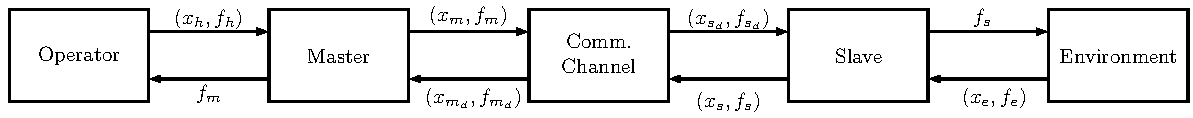
\includegraphics[width=\textwidth]{schemas/Bilateral_Teleop.pdf}
	\caption[Block representation of the bilateral teleoperation]{Block representation of the bilateral teleoperation.}
	\label{sch:bilateral_teleop}
\end{figure}
At each side, master and slave, a local controller is implemented that combines local and remote information to create a bilateral coupling: the operator actuates the slave while feeling a force feedback from the remote site.\\
The communication channel could be affected by delays: this means that a command sent from the master at time $t$ is received by the slave at time $t + \tau_{m2s}$, where $\tau_{m2s}$ is the amount of time required to transmit the information in the feed forward channel.\\
Consequently a feedback produced by the slave at time $t$ is received at the master at time $t+ \tau_{s2m}$, with $\tau_{s2m}$ the amount of time required to transmit the information in the feedback channel. The sum of  $\tau_{m2s}$ and $\tau_{s2m}$ is denoted as \textit{round-trip time} delay.\\
A good bilateral teleoperation system should ensure the operator a transparent and stable interface with the environment, allowing safe and immediate responses to any event both known and unknown.\\
From a theoretical point of view, the two main properties for a bilateral teleoperation system are:
\begin{description}
	\item[Stability] The system should maintain the stability of the closed control loop independently of operator's or environment's behaviour. Stability of the whole system is hard and complex to prove, thus this property is more easily investigate with the passivity theory.
	\item[Transparency] Is the capability of the system to provide to the operator the sense of telepresence while interacting with the remote environment. 
\end{description}

\section{Stability}
There is no single concept of stability, and many different definitions are possible.
The following are fundamental statements for stability:
\begin{definition}
	An equilibrium state $x=0$ is said to be:
	\begin{enumerate}[label=(\alph*)]
		\item \emph{\textbf{Stable}} if for any positive scalar $\varepsilon$ there exists a positive scalar $\delta$ such that $\norm{x(t_{0})} < \delta$ implies $\norm{x(t)} < \varepsilon$ for all $t \geq t_{0}$.
		\item \emph{\textbf{Asymptotically stable}} if it is stable and if in addition $x(t) \rightarrow 0$ as $t \rightarrow \infty$
		\item \emph{\textbf{Unstable}} if it is not stable.
	\end{enumerate}
\end{definition}
The definition (a) is often called “stability in the sense of Lyapunov” (stability i.s.L.) after the Russian mathematician Aleksandr M. Lyapunov (1857- 1918), whose important work features prominently in current control theory.
Asymptotic stability in the large implies that all motions are bounded.
Generally,
\begin{definition}
	An equilibrium state $x=0$ is said to be \textbf{bounded} (or Lagrange stable) if there exists a constant $M$, which may depend on $t_{0}$ and $x(t_{0})$, such that $\norm{x(t)} \leq M$ for all $t \geq t_{0}$.
\end{definition}

To provide a proof of passivity the aim is to determine the stability nature of the equilibrium state (at the origin) of system $\varSigma$ without obtaining the solution $x(\cdotp)$.
This could be done with the so called \textit{direct method of Lyapunov} in relation to the (initialized) nonlinear autonomous dynamical system
$\varSigma$ given by
\begin{equation}\label{Lyapunov_system}
	\dot{x} =F(x),\quad x(0)=x_{0} \in \mathbb{R}^{n}; \quad F(0)=0 
\end{equation} 
Modifications needed to deal with the (non autonomous) case 
\[ \dot{x}  = F ( t , x ) , \quad x ( t_{0} ) = x_{0} \]
are possible.

The essential idea is to generalize the concept of energy $V$ for a conservative system in mechanics, where a well-known result states that an equilibrium point is stable if the energy is minimum.
\\Thus $V$ is a positive function which has $\dot{V}$ negative in the neighbourhood of a stable equilibrium point.\\
More generally,
\begin{definition}
	We define a Lyapunov function $V : \mathbb{R}^{n} \rightarrow  \mathbb{R}$ as follows :
	\begin{itemize}
		\item  $V$ and all its partial derivatives $\dfrac{\partial V}{\partial x_{i}}$ are continuous
		\item V is positive definite; that is, $V(0)=0$ and $V(x)>0$ for $x\neq0$ in
		some neighbourhood $\{x \mid \norm{x} \leq k\}$ of the origin
	\end{itemize}
\end{definition}

A Lyapunov function $V$ for the system \eqref{Lyapunov_system} is said to be
\begin{itemize}
	\item \textbf{strong} if the derivative $\dot{V}$ is \textit{negative definite};\\ that is, $\dot{V}(0) = 0$  and $\dot{V}(x)<0$ for $x\neq0$ such that $\norm{x}\leq k$.
	\item \textbf{weak} if the derivative $\dot{V}$ is \textit{negative semi-definite};\\that is, $\dot{V}(0) = 0$ and $\dot{V}(x)\leq0$ $\forall x$ such that $\norm{x}\leq k$.
\end{itemize}

The statements of the two theorems of Lyapunov are :
\begin{theorem}
	\emph{\textbf{Lyapunov’s First Theorem}}\\ Suppose that there is a strong Lyapunov function $V$ for system $\varSigma$. Then system $\varSigma$ is asymptotically stable.
\end{theorem}
\begin{theorem}
	\emph{\textbf{Lyapunov’s Second Theorem}}\\  Suppose that there is a weak Lyapunov function $V$ for system $\varSigma$. Then system $\varSigma$ is stable.
\end{theorem}
\section{Passivity}
One method derived from control theory to ensure stability of the whole teleoperation system, even in presence of delays, is by designing each component in a way that it is passive.\\
By the definition found in \cite{Lozano200}, a system $G(s)$ is passive if and only if a finite amount of energy can be extracted from it; or, in other words, the energy that can be extracted by a passive system is always less or at most equal to the amount inserted. 
Intuitively, a passive teleoperation system cannot increase the amount of energy inserted in it by the operator and/or by the environment.\\
To introduce the required formulation of passivity, the following definition of extended measurable functions is needed:
\begin{definition}
	Let $\mathcal{L}_{2}(\mathbb{R}^{n})$ be the space of all measurable function $f$ : $\mathbb{R} \rightarrow \mathbb{R}^{n}$ for which
	\begin{equation}
	\int_{-\infty}^{+\infty} \norm{f\left( t\right) }^{2} dx < \infty
	\end{equation}
\end{definition}
\begin{definition}
	The space $\mathcal{L}_{2e}(\mathbb{R}^{n})$, $\mathcal{L}_{2}(\mathbb{R}^{n})$ extended, is defined as the space of all measurable function $f$ : $\mathbb{R} \rightarrow \mathbb{R}^{n}$ for which
	\begin{equation}
		f_{T} \in \mathcal{L}_{2}(\mathbb{R}^{n}) \quad \forall T\in\left[ -\infty,+\infty \right] 
	\end{equation}
\end{definition}
where $f_{T}$ is the truncated version of $f$.
Then the passivity definition, as in \cite{Anderson1989}, is the following:
\begin{definition}
	If the input in the time domain is described as $u(t) \in \mathcal{L}_{2e}(\mathbb{R}^{n})$ and the output $y(t) \in \mathcal{L}_{2e}(\mathbb{R}^{n})$,\\
	a system
	\[G :  \mathcal{L}_{2e}(\mathbb{R}^{n}) \rightarrow \mathcal{L}_{2e}(\mathbb{R}^{n}) \quad u \rightarrow v = G(u)\]
	is passive if there exist a constant $\beta > 0$ such that
	\begin{equation}
		\int_{0}^{t}y^{T}(\tau)u(\tau) d\tau\geq-\beta \quad\quad\forall t \geq0, \forall u\left( \cdotp \right) 
	\end{equation}
\end{definition}
The combination of two passive systems, connected in a feedback or parallel configuration, is a passive system as well.
The connection of passive systems in a series configuration may not result in a passive system.\\
To show that passivity implies stability, we recall the definition of stability for a linear, time-invariant system $G(s)$ performed by the analysis of poles and zeroes of the system's transfer function in the Real and Imaginary plane.
\begin{definition}
	 A linear, time-invariant system $G(s)$ is defined \textbf{stable} if and only if it does not present any pole in $\mathbb{R}^{+}$ plane and the poles in  $\mathbb{R}^{0}$ are simple.
\end{definition}
The previous considering the imaginary axis and  excluding  $\mathbb{R}^{+} \cup \mathbb{R}^{0}$ plane result in the \textbf{asymptotical stability} definition.
The following theorem conveys these formulations for passivity and stability, proving that the former implies the latter:

\begin{theorem}
	Let $G(s)$ be the transfer function of a linear, time-invariant (LTI), single input/single output (SISO) system. G(s) is passive if and only if
	\begin{itemize}
		\item $G(s)$ has no pole in the $\mathbb{R}^{+}$ plane
		\item  $ReG(j\omega) \geq 0,\quad \forall\omega \in [−\infty, +\infty]$ such that $j\omega$ is not a pole for $G(s)$
		\item if $j\omega_{0}$ is a pole of $G(s)$, then it must be simple and the residual be greater than 0
		\[\lim(s − j\omega_{0})G(s) \geq 0\]
	\end{itemize}
\end{theorem}

\section{Teleoperation without delay}
Most teleoperation algorithms has been designed to be robust even in an environment were communication delays occur.
Despite that, some critical applications require absolute stability and high reliable network conditions.

\subsection{The Four Channel Architecture}
A solution, namely \textit{The Four channel Architecture} was proposed by Lawrence \cite{Lawrence1993}.\\
It's a PF-PF (Position Force) architecture using forces and velocities as reference signals.

The teleoperation system is completely transparent if the operator feels that is
directly interacting with the remote environment: this implies equality between  forces $(F_{m} = F_{s})$ and velocities $(V_{m} = V_{s})$.\\
Transparency requires that the transmitted impedance $Z_{t}$ is equal to the
environment impedance $Z_{e} = F_{s}$. According to the block diagram in \figurename{\ref{sch:Four_channel}} the controllers $C_{s},C_{m},C_{1}, \dots C_{4}$ have to be designed in such a way that the hybrid matrix $H$
\begin{figure}
	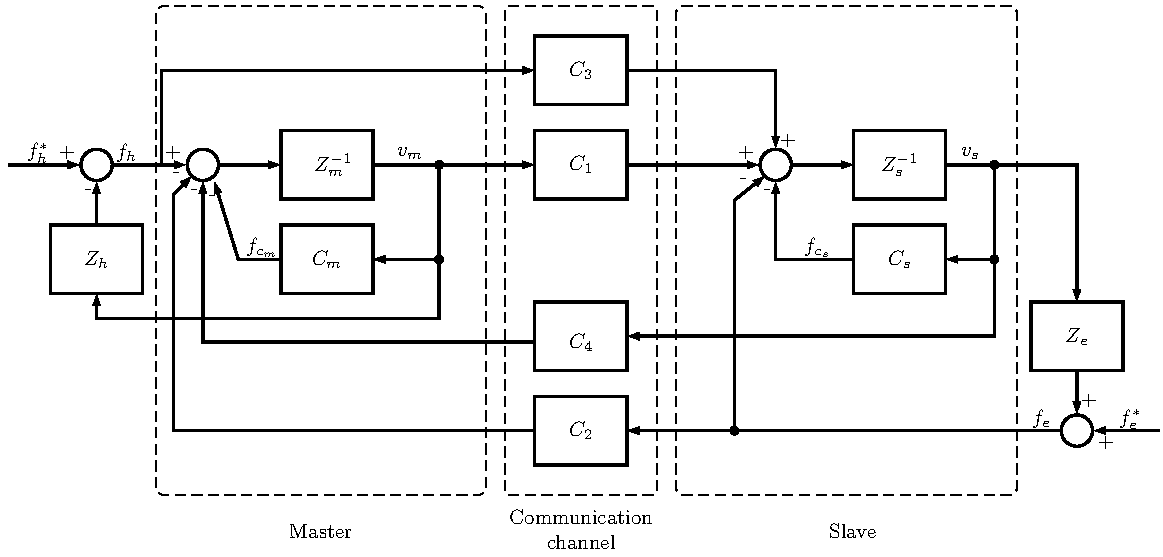
\includegraphics[width=\textwidth]{schemas/Four_channel.pdf}
	\caption[The Four Channel Architecture]{The Four Channel Architecture.}
	\label{sch:Four_channel}
\end{figure}
\begin{equation}
	\begin{bmatrix}
		F_{m}(s)\\
		V_{m}(s)
	\end{bmatrix}
	= 
	\underbrace{
		\begin{bmatrix}
			H_{11}(s) & H_{12}(s)\\
			H_{21}(s) & H_{22}(s)
		\end{bmatrix}
	}_{\text{$\triangleq H$}}
	\begin{bmatrix}
		V_{s}(s)\\
		F_{s}(s)
	\end{bmatrix}
\end{equation}
is equal to $\begin{bmatrix} 0 & I\\ I & 0 \end{bmatrix}$.\newpage
\noindent That implies
\begin{equation}
	Z_{t} = \dfrac{F_{m}}{V_{m}} = \left( H_{11} -H_{12}Z_{e}\right) \left(  H_{21} -H_{22}Z_{e}\right)^{-1} = Z_{e}
\end{equation}
To achieve the goal of transparency, it is necessary to have a very accurate model both of master and slave robots.
A good transparency is required mainly at low frequencies, where mathematical models are more accurate, in order to provide a good feedback at frequencies the operators work on.
In his work, Lawrence proposes to associate the abstract notion of passivity derived from the mathematical representation of positive real transfer functions to a more physical measure of passivity that describes how the covariant variables at each port must be in phase in order to maintain a positive energy flow to the system.

\section{Teleoperation with constant delay}
The transmission of power variables over a communication channel affected by delays, is the reason for which bilateral teleoperation models may become unstable.
Consider a basic control system structure, the mathematical description clearly shows the effect of the delays over the communication channel. Considering an input and output $X(s)$, $Y(s)$ in the Laplace domain variable $s$, a plant $P(s)$, a controller $C(s)$ and a feedback delay of $T$ seconds, the transfer
function of $G(s)$ is:
\begin{equation}
	G(s) = \dfrac{Y(s)}{X(s)} = \dfrac{e^{sT}P(s)C(s)}{1+e^{sT}P(s)C(s)}
\end{equation}
The term $e^{sT}$ that appears at denominator is the cause of the performance loss. Increasing the value of $T$, the system loses phase margin, thus the system could become unstable.\\
With a passivity based analysis the communication channel could be separated from the master and slave blocks allowing the demonstration of system's stability by passivating the channel.

\subsection{PD and passivity terms}
Lee and Spong \cite{Lee2006} provides a solution for the teleoperation with constant time delay. It guarantees the stability of a position-position bilateral teleoperator by adding a dissipative term to the PD controller at each side of the architecture.
\begin{figure}
	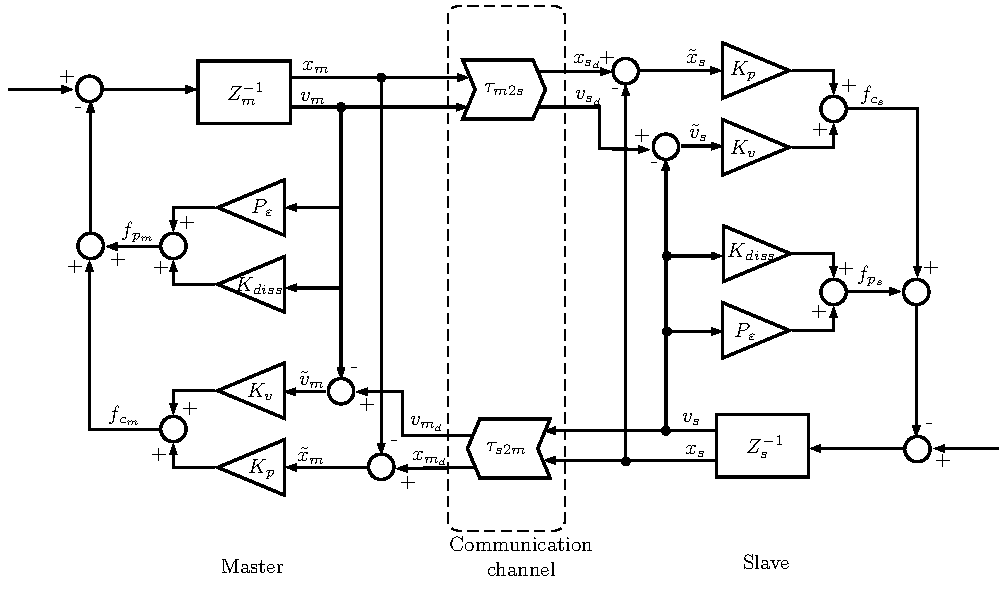
\includegraphics[width=\textwidth]{schemas/Lee-spong.pdf}
	\caption[Lee-Spong PD dissipative approach]{Lee-Spong PD dissipative approach }
	\label{sch:Lee_spong}
\end{figure}
 \figurename{ \ref{sch:Lee_spong}} shows the block-schema of this architecture.
This solution does not suffer of position drift between master and slave, which is the major drawback of scattering-based solutions due to the extraction of velocity from the communicated scattering variables \cite{Lee2006}.\\
The explicit position feedback enables to guarantee the asymptotic master-slave position coordination.
This approach passifies the combination of the communication and control blocks all together, in contrast to scattering approach, where the delayed communication block is passified in such a way that the closed-loop teleoperator becomes an interconnection of passive submodules.
Stability is guaranteed by an over estimation of the round-trip time delay $\bar{\tau}_{RTT} \geq \tau_{RTT}$.\\
Representing a manipulator with:
\begin{equation}
	M(q)\ddot{q}(t) + C(q,\dot{q})\dot{q} = T(t) + F(t)
\end{equation}
where $q \in \mathbb{R}^m$ is the configuration, $F \in \mathbb{R}^n$ is the interacting force, $T \in \mathbb{R}^n$ the control, $M(q)  \in \mathbb{R}^{m\times m}$ the symmetric and positive-definite inertia matrix and $C(q,\dot{q}) \in \mathbb{R}^{m \times m} $, the control terms for master and slave could be written as function of local and remote delayed informations as follow:
\begin{align}\label{lee_spong_mcommand}
	T_{m}(t)&:=  T_{m} \left( q_{m}(t), \ \dot{q}_{m}(t), \ q_{s}(t - \tau_{s}), \ \dot{q}_{s}(t - \tau_{s})  \right) \in \mathbb{R}^m \\
	\label{lee_spong_scommand}
	T_{s}(t)&:= T_{s}\left( q_{s}(t), \ \dot{q}_{s}(t), \  q_{m}(t - \tau_{m}), \ \dot{q}_{m}(t - \tau_{\textsf{m}})  \right) \in \mathbb{R}^m
\end{align}
The goal is to design the control terms $T_{s}$ and $T_{m}$ to achieve
\begin{itemize}
	\item \textbf{master-slave position coordination} if $(F_{m},F_{s} )= 0$, then
	\begin{equation}\label{lee-sopong_pos}
		q_{error}(t):= q_{m}(t) - q_{s}(t) \rightarrow0, \quad t\rightarrow 0
	\end{equation}
	\item  \textbf{static force reflection} if $(\dot{q}_{m}(t),\  \dot{q}_{s}(t), \ q_{m}(t), \ q_{s}(t)) \rightarrow 0$, then
	\begin{equation}\label{lee-sopong_force}
	F_{m}(t) \rightarrow -F_{s}(t)
	\end{equation}
	\item \textbf{energetic passivity} of the closed loop teleoperation system. It there exists a finite constant $d \in \mathbb{R}^m$ such that
	\begin{equation}\label{lee-sopong_passivity}
	\int_{0}^{t}\left[ F^{T}_{m}(\theta) \dot{q}_{m}(\theta)+ F^{T}_{s}(\theta) \dot{q}_{s}(\theta)\right] d\theta \geq d^{2} \quad \forall t\geq 0
	\end{equation}
	meaning that the maximum extractable energy from the two-port closed-loop teleoperator is always bounded.
\end{itemize}
In order to fulfil \eqref{lee-sopong_pos}, \eqref{lee-sopong_force} and \eqref{lee-sopong_passivity}
the design of master and slave controls $T_{m}(t)$ and $T_{s}(t)$ in \eqref{lee_spong_mcommand} and \eqref{lee_spong_scommand} is:
\begin{multline}
	T_{m}(t) = \underbrace{
						\underbrace{
							-K_{p}((q_{m}(t) - q_{s}(t-\tau_{m}))
						}_{\text{delayed P-action}}
						\underbrace{
							-K_{v}(\dot{q}_{m}(t) - \dot{q}_{s}(t-\tau_{m})
						}_{\text{delayed D-action}}
					}_{F_{mc}}\\
					\underbrace{
						\underbrace{
							-\left( K_{d}+P_{\varepsilon}\right)(\dot{q}_{m}(t))
						}_{\text{dissipation}}
					}_{F_{mp}
				}
\end{multline}
\begin{multline}
	T_{s}(t) = \underbrace{
		\underbrace{
			-K_{p}((q_{s}(t) - q_{m}(t-\tau_{s}))
		}_{\text{delayed P-action}}
		\underbrace{
			-K_{v}(\dot{q}_{s}(t) - \dot{q}_{m}(t-\tau_{s})
		}_{\text{delayed D-action}}
		}_{F_{sc}}\\
		\underbrace{
			\underbrace{
					-\left( K_{d}+P_{\varepsilon}\right)(\dot{q}_{s}(t))
			}_{\text{dissipation}}
		}_{F_{sp}}
\end{multline}
where $K_{d}= \dfrac{\bar{\tau}_{RTT}}{2} K_{p}$ and $P_{\varepsilon}$ is an additional damping ensuring master-slave coordination.
\section{Teleoperation with time varying delay} 
The occurrence of time-varying delays makes the energy handling in the communications channel a challenging problem.
Even the most stable and transparent architecture is susceptible to that.\\
The simpler solution is the use of buffers at each side to re-order information and absorb the variation by releasing packets with a constant rate.
The drawbacks of this approach are the increased RTT because of the time spent for store each packet in the buffer and the dynamic growing of the buffer if the delay increases.
\subsection{PSPM}\label{PSPM}
The Passive Set-Position Modulation (PSPM) is P-P teleoperation architecture proposed by Lee \cite{Lee2010} that addresses teleoperation with time-variant delay.\\
\begin{figure}
	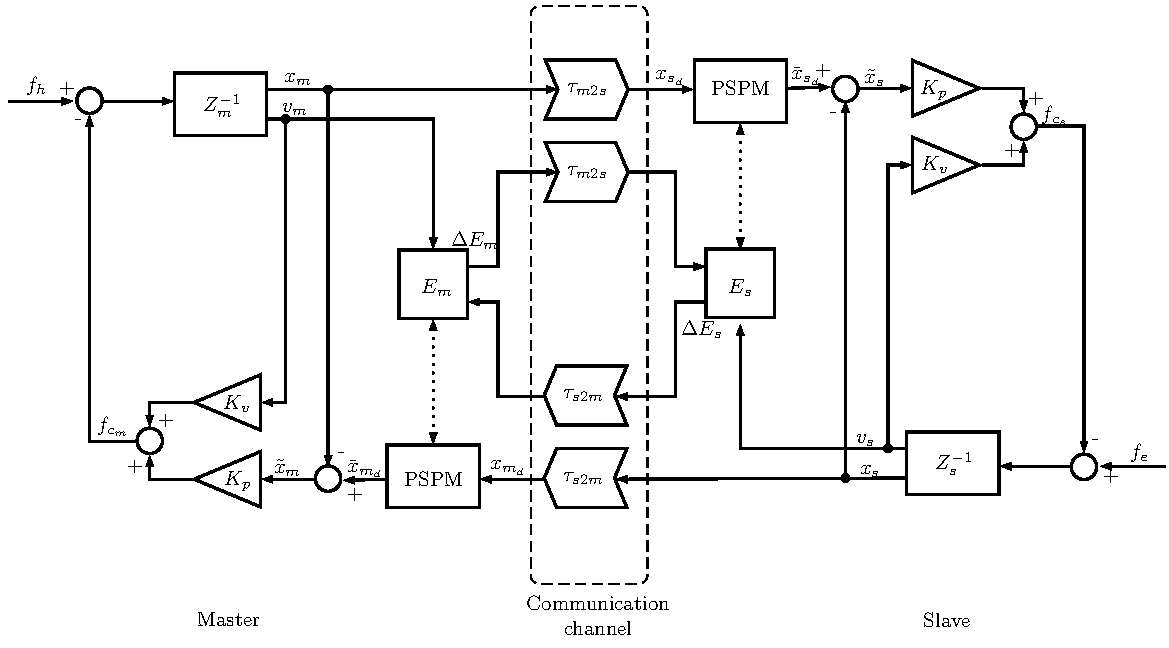
\includegraphics[width=\textwidth]{schemas/PSPM.pdf}
	\caption[PSPM teleoperation schema]{PSPM teleoperation schema}
	\label{sch:PSPM}
\end{figure}
A representation is available in \figurename{ \ref{sch:PSPM}}
The input signal $y(k)$ is a discrete-time input sequence of sparse or slowly updating set position, possibly non uniformly received at time $t_{k}$. \\
This signal is applied to a spring-damper model $K_{P}\left( x(t) - y(k) \right) + K_{d}v(t)$ where $x(t)$ and $v(t)$ are the continuous time values of manipulator position and velocity.
The approach consider the possible passivity breaking due to the spring's energy jump at switching instances by solving the minimisation problem
\begin{equation}
	\norm{x(t) - y(k)} \quad \text{s.to} \quad E(k+1) + \Delta E_{in}(k) + D(k-1) -\Delta \bar{P}(k) \geq 0
\end{equation}
 into the PSPM block each time the reference signal is updated.
 $E(k+1)$ is the local energy reserve , $\Delta E_{in}(k)$ is the energy received at time $t_{k}$ from the counterpart (\textit{energy-shuffling}), $D(k-1)$ is the causal approximation of the damping dissipation (\textit{energy re-harvesting}), namely $\dfrac{1}{2}K_{d}v^{2}(t)$, that is position-only dependent to avoid the sequence of numerical differentiation and integration that will introduce noise contamination into the signal. Finally $-\Delta \bar{P}(k)$ is the spring energy jump
 \begin{equation}
 	-\Delta \bar{P}(k) = \dfrac{1}{2}\norm{x(t_{k}) - \bar{y}(k)}^{2}_{K_{p}} - \dfrac{1}{2}\norm{x(t_{k}) - \bar{y}(k-1)}^{2}_{K_{p}}
 \end{equation}
 The resulting $\bar{y}(k)$ signal is modulated in such a way that it is as close as possible to the original $y(k)$ yet only to the extent that the use of $\bar{y}(k)$ for the spring coupling $K_{p}$ is permissible by the passivity constraint.\\
 The \textit{virtual energy reservoir} is a mechanism to improve performance by the use of \textit{energy reharvesting}. It recaptures and deposits in the \textit{energy reservoir}  a portion of the otherwise wasted energy due to the damper and through the \textit{energy shuffling/ceiling}. The latter limits the accumulation of virtual energy by setting an upper shorthold to the reservoir and sending the exceeding energy to the counterpart.
 
 This approach should accommodate a variety of communication/data-update imperfections of $y(k)$, including variable-rate update, varying delay, packet loss, and even time-swapping.
 
 \subsection{The Two Layer Algorithm}\label{Two-Layer-Approach}
This algorithm proposed by Franken \textit{et al.} \cite{Franken2011} implements a hierarchical two-layer approach: a top \textit{transparency layer} and a bottom \textit{passivity layer}.
The main idea is that, without making any assumption about on type of controller implemented, in the former layer a control algorithm is in charge of displaying the desired behaviour and achieving transparency. The only requirement is that the algorithm implemented in this layer computes the control forces $\tau_{TL}$ to be applied to the manipulator.\\
The passivity layer on the bottom monitors and enforces the energy balance in the system ensuring that no virtual energy is generated.
With this approach, the strategy used to obtain transparency is independent  of the one to obtain passivity, thus enabling the possibility to adopt in the transparency layer strategies known to be non passive e.g. most filtering techniques.\\
Two two-way communication channels enable the communication between master and slave: one is dedicated to communicate energy exchange information between the passivity layers, the other relays the information required by the algorithm in the transparency layer.
\begin{figure}
	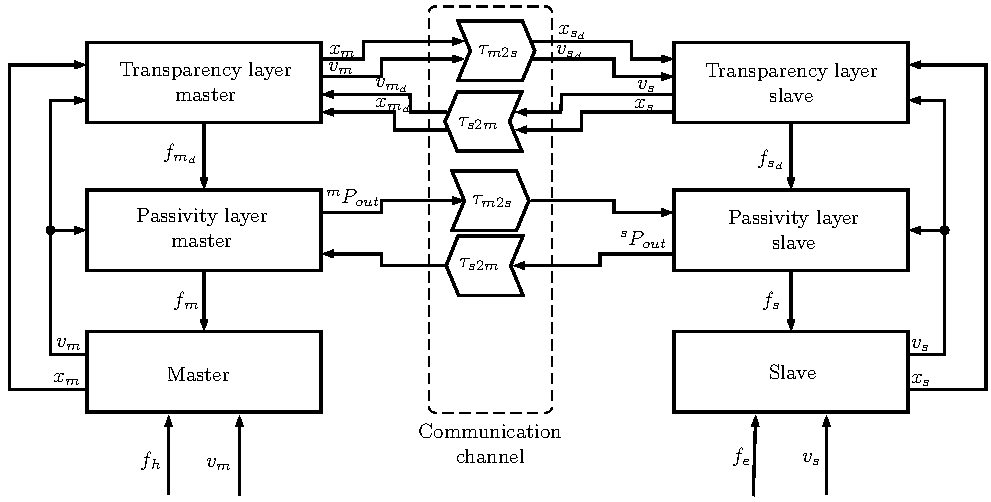
\includegraphics[width=\textwidth]{schemas/TwoLayer.pdf}
	\caption[TwoLayer teleoperation schema]{TwoLayer teleoperation schema. $F_{m_{d}},F_{s_{d}}$ are master and slave $\tau_{TL}$, while $f_{m}, f_{s}$ are the two $\tau_{PL}$}
	\label{sch:TwoLayer}
\end{figure}
In contrast with other approaches, the passivity is achieved after the computation of the commands and not before. This architecture is summarized in \figurename{\ref{sch:TwoLayer}}.

The passivity layer requires impedance causality both for master and slave (i.e. velocities as input and forces as output).\\
The latter layer acts as follows: at first, the energy exchange between the discrete time controller and physical world is evaluated as:
\begin{equation}
	\begin{split}
		\Delta H(k) & = \int_{(k-1)\Delta T_{s}}^{(k)\Delta T_{s}} \tau_{r}(k)\dot{q}(t)dt\\
		& =	\tau_{r}(k)(q(k)-q(k-1))\\
		& =\tau_{r}(k) \Delta q(k)
	\end{split}
\end{equation}
where $\tau_{r}(k)$ is the torque exerted by the actuators at sample $k$, $\dot{q}(k)$ the velocity vector of the actuators and $q(k)$ their sampled position.\\
At the same time the energy received from the counterpart is taken into account:
\begin{equation} 
	H_{+}(k) = \sum_{i\in Q(k)}H(i)
\end{equation}
where $Q$ is the queue which stores all the packets received between two time instants and $H(i)$ is the $i_{th}$ packet in the queue.
Then the energy level in the local tank is updated:
\begin{equation}
	H(k)= H(\bar{k}) + H_{+}(k) - \Delta H(k)
\end{equation}
where $H(\bar{k})$ is the state of the tank at the previous sampling time.\\
An energy quantum $H_{-}(k) < H(k)$ could be transferred to the tank on the other side of the teleoperation system according to the transport protocol that has been implemented. $H_{-}(k)$ is then extracted from the tank.
The energy available during the next sampling period 	$H(\overline{k+1})$ becomes
\begin{equation}
	H(\overline{k+1}) = H(k) - H_{-}(k)
\end{equation} 
The available energy is then used to ensure the stability of the system.\\
An approach could be to allow the command $\tau_{TL}$ only if the tank stores enough energy
\begin{equation*}
		\tau_{max1}(k) =
	\begin{cases}
	0, & \mbox{if } H(\overline{k+1})  \leq 0\\
	\tau_{TL}, & \mbox{otherwise}
	\end{cases}
\end{equation*}
or to compute an upper bound for the command in order to guarantee the stability of the teleoperated system
\begin{equation*}
	\tau_{max2}(k) = \dfrac{H (\overline{k+1})}{\dot{q}(\bar{k}) \Delta Ts}.
\end{equation*}
The combination of multiple approaches allows more advanced passivation strategy by allowing e.g. the minimum value from a set of conditions
\begin{equation*}
	\tau_{max}(k) = \min(\tau_{max1}(k),\tau_{max2}(k),\dots)
\end{equation*}
Then the torques $\tau_{PL}$ are a bounded version of the ones requested by the transparency layer
\begin{equation}\label{tau_TL}
\tau_{TL}(k) = sgn(\tau_{TL}) \min(\tau_{PL},\tau_{max}(k)).
\end{equation}
To maintain the energy level above a minimum threshold, usually at master side, a Tank Level Controller (TLC) is implemented.
When the energy goes below the threshold $H_{D}$, an extra variable damping is injected to extract an extra amount of energy
\begin{equation}
	\tau_{TLC}(k) = -d(k)\dot(q)(k)
\end{equation}
with $d(k)$
\begin{equation}
		d(k) = 
		\begin{cases}
			\alpha(H_{D} - H(\overline{k+1})), & \mbox{if } H(\overline{k+1})  < H_{D}\\
			0, & \mbox{otherwise}
		\end{cases}
\end{equation}
Thus the command to be applied to the device during the sample period $k+1$ becomes
\begin{equation}
\tau_{r}(k+1) = \tau_{TL}(k) + \tau_{TLC}(k)
\end{equation}
Looking at the communication channel, the change of energy in the channel $\Delta H_{C}(k)$ at sample $k$ is
\begin{equation}
	\begin{split}
		H_{C}(k) & = \sum_{i=1}^{k} \Delta H_{C}(k)\\
		& = \sum_{i=1}^{k} H_{-M}(i) - H_{+M}(i) + H_{-S}(i) + H_{+S}(i) 
	\end{split}
\end{equation}
and due to time delays and packet loss in the channel 
\begin{equation*}
	H_{-S}(i) = H_{+M}(i+d_{SM}(i))
\end{equation*}
\begin{equation}
H_{-M}(i) = H_{+S}(i+d_{MS}(i))
\end{equation}
where $d_{MS}(i)\geq 0$ and $d_{SM}(i)\geq 0$ takes into account nondeterministic time delays.
Therefore 
\begin{equation}
	\begin{split}
		\sum_{i=0}^{k} H_{-M}(i) & \geq \sum_{i=0}^{k} H_{+S}(i)\\
		\sum_{i=0}^{k} H_{-M}(i) & \geq \sum_{i=0}^{k} H_{+S}(i)
	\end{split}
\end{equation}
so that
\begin{equation}
H_{C}(k) \geq 0 \qquad \forall k
\end{equation}
meaning that the communication channel can never produce energy as long as packets duplication is prevented.\\
We can now write the total energy $H_{T}(k)$ in the control system at instant $k$ as 
\begin{equation}
	H_{T}(k) = H_{M}(k) + H_{C}(k) + H_{S}(k).
\end{equation}
Finally the passivity condition for the system is 
\begin{equation}
H_{T}(k) \geq 0
\end{equation}
and the condition that ensure a passive interconnection of the entire system to the physical world is
\begin{equation}\label{Two_layer_passivity_world}
	\dot{H}_{T}(k)\leq P_{M}(k) + P_{S}(k)
\end{equation}
where $\dot{H}_{T}(k)$ is the rate of the energy balance of the system, $P_{M}(k)$ and $P_{S}(k)$ are respectively the power of master and slave flowing between the robot and it's respective controller.

\section{Discussion}
In this chapter the problem of teleoperation has been addressed and some of the possible solutions to overcome the problem of delay in the communication and keep the system passive have been presented.
Teleoperation have two main goals: stability and transparency. The former is mandatory and ensured by the passivity of the system, the latter is responsible for a good haptic feedback and for the precision while performing a task.\\
The strategy adopted to achieve the goal of passivity could reduce the level of transparency in the system. A flexible and robust approach between the one presented is the Two-Layer algorithm. 


\clearpage
\thispagestyle{empty}